\chapter{Transcription regulation}

Multicellular organisms, such as human, are formed by thousands of cell types. However, the genome in every of those cells is identical. If the recipe is the same, how is it possible to have so many cells types that manage to work together and run such a complex organism? The expectation of the Human Genome project was that once we have a complete sequence of the genome, it will be fairly straightforward to solve the causes of diseases, easier to understand human evolution and development. But as it turned out, the majority of the human genome (98\%) does not code for proteins, but nevertheless is essential for the regulation of all expressed genes \cite{pang2023identification}. The genome is much more mysterious, and we are still studying its complexity \cite{kumar2016human}.

Processes that are not directly associated with the DNA sequence, are responsible for controlling the genome and its gene expression. Such mechanisms are termed as epigenetic mechanisms (epi- means "over, outside") \cite{jablonka2002changing}. DNA methylation, histone tail modifications, micro RNA are all contributing to the regulation of gene expression transcription regulation \cite{mitsis2020transcription}. Genomic DNA is constantly being approached by regulatory proteins and other small molecules. The major players in transcriptional regulation are \ac{TFs}. Without TFs RNA polymerase and the basic transcriptional machinery would not be able to approach genes and begin transcription. TFs act in different modes and are able to find and bind regulatory regions --- promoters and enhancers. Bound TFs attract Mediator proteins and Pol II and form a loop that brings enhancers and promoter regions close in space even though they can be separated by kilobases in a linear space ({Figure \ref{regions_loop}}). The activation of gene expression is tightly regulated and is cell type- and time-specific.

\begin{figure}
  \centering
  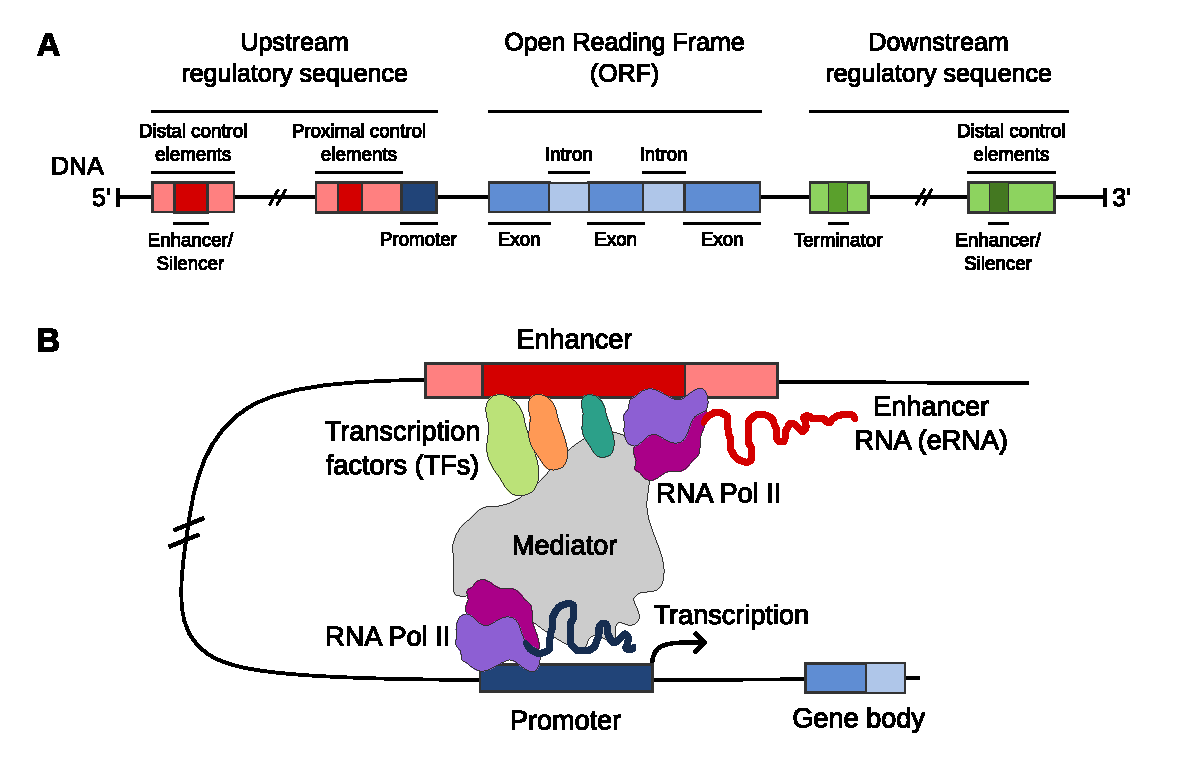
\includegraphics[width=1\textwidth]{figures/regulatory_regions/regulation_latest.pdf}
  \caption[Regulatory regions and transcription regulation]{\textbf{Transcription is regulated through protein binding to the gene cis-regulatory regions.} \textbf{A.} Regulatory regions can be found upstream and downstream of the gene body (open reading frame). Regulatory sequences can be in a close proximity (proximal) or separated by numerous bases (distal). Distal regulatory regions are enhancers and silencers. \textbf{B.} For transcriptional machinery to know which gene needs to be transcribed, transcription factors (TFs) are binding enhancers, which stimulates the binding of Mediator proteins and subsequently RNA polymerase II (Pol II). The binding brings enhancer and promoter regions closer in space and transcription starts. RNA Pol II proteins transcribes a gene into pre-mRNA, but also produces enhancer RNA (eRNA). Modified from \cite{wu2019super,villao2023plant,wasserman2004applied}.}
  \label{regions_loop}
\end{figure}

  \section{Cis-regulatory regions}

  Regulatory regions in the eukaryotic genome are segments of the DNA that are associated with capability to increase or decrease the transcription. These regions are termed \ac{CRRs}. They are crucial for gene expression regulation, because they contain a set of short DNA sequences, \ac{TFBSs}, which are targeted by TFs \cite{wasserman2004applied}. CRRs include promoters, enhancers and silencers.

    \subsection{Promoters}

    Promoters are located at the 5' end region of the gene ({Figure \ref{regions_loop}}A) and are crucial for gene expression regulation. Core promoters are located 40 bp upstream or downstream from the transcription start site (TSS) and are minimal regions needed for transcription initiation \cite{haberle2016promoter,kadonaga2012perspectives}. Promoters have specific DNA sequence elements important for gene regulation. For example, TATA box element in the core promoter is bound by TBP, the Initiator sequence is one of the most common elements and encompasses the +1 TSS, while different sequence motifs can be bound by specific TFs \cite{villao2023plant,wasserman2004applied,haberle2016promoter,kadonaga2012perspectives}. Another characteristic common for human promoters is the abundance of CpG dinucleotides. CpGs are targets for cytosine methylation, which is one of the gene regulatory mechanisms \cite{wasserman2004applied,saxonov2006genome}. Around 70\% of human promoters near TSSs contain a \ac{CGI}, which is a region with high frequency of CpGs \cite{deaton2011cpg,saxonov2006genome,haberle2016promoter}.

    Based on promoter composition, nucleosome positioning and what genes they regulate, promoters can be classified into four main types: type I, II, III and IV \cite{haberle2016promoter}. Type I promoters are adult tissue-specific and their transcription starts at the precise position. These promoters have a TATA box around 30 bp upstream from the TSS and nucleosome are distributed in a disordered fashion along the sequence. Type II promoters are controlling the expression of the housekeeping genes and transcription can be initiated at the several locations. Type III promoters regulate developmental genes and also have a broad initiation pattern. Interestingly, these promoters depend on the input from distal enhancers. Type IV promoters are transcriptional machinery-specific and, like type I, have a sharp transcription initiation pattern. In type II, III and IV promoters there is a nucleosome-free region with precisely positioned two nucleosomes downstream and upstream. In addition, all three types of promoters have CGIs covering the TSSs \cite{haberle2016promoter}.

    \subsection{Enhancers and silencers}

    Enhancers are distal regulatory regions that activate transcription by acting on a promoter over large genomic distances ({Figure \ref{regions_loop}}) \cite{smith2014enhancer}. The distance from enhancer to the promoter it acts on can vary from several kilobases to megabases \cite{field2020evaluating,karpinska2023role}. The size of enhancers also varies from less than 100 bp long elements to 10--100 kb sequences, which are sometimes referred to as super-enhancers \cite{field2020evaluating,hnisz2013super,smith2014enhancer}. They often act in a spatially and temporally restricted manner, which means that enhancers are cell-type specific and are active only at the specific time points \cite{field2020evaluating}. Enhancers are approached by transcription factors and bind specific DNA patterns. Multiple TFs can bind one enhancer, depending on how many potential TFBSs that enhancer has \cite{wu2019super,field2020evaluating}. Fairly recently it has been discovered that enhancer DNA is being transcribed into non-coding RNA, termed \ac{eRNA} ({Figure \ref{regions_loop}}B) \cite{smith2014enhancer}. These RNAs are promoting the functions of enhancers by recruiting TFs, promoting enhancer-promoter looping, influencing chromatin conformation or histone acetylation status \cite{wu2019super,field2020evaluating}.

    Enhancer-promoter loops are supported by cohesin. Cohesin is a ring-like structure that holds the loop together letting enhancer and promoter communicate through complexes of proteins \cite{smith2014enhancer,field2020evaluating}. Formation of loops is known as loop extrusion. Another loop-extruding factor is protein CTCF. It binds DNA at the borders of the loop, this way informing cohesin where to hold the loop. It is described as insulating a particular region \cite{field2020evaluating}. Influence of the enhancers is most of the time, but not always, limited to the genes that are within the same loop \cite{karpinska2023role,luppino2020cohesin,symmons2014functional}. One enhancer can regulate multiple genes, while one gene can be regulated by multiple enhancers. The compartments where transcription regulation is self-contained are known as \ac{TADs}. Multiple loops can be found in one TAD \cite{karpinska2023role,luppino2020cohesin}.

    Opposite to the enhancers, silencers are DNA sequences that are bound by the repressor proteins in order to silence gene transcription \cite{spitz2012transcription}. Even though most of the research is focused on enhancer and promoter identification, silencers are interesting and important regions to research. It is known that silencers can also be tissue-specific and that they operate within TADs through short- or long-range interactions \cite{pang2020systematic,pang2023identification}. These regions are marked by specific chromatin marks, such as \ac{H4K20me} \cite{pang2020systematic,beck2012pr}. Silencers are targeted by repressive TFs and through looping communicate with the promoter of the gene, which expression needs to be repressed \cite{pang2023identification}.

  \section{Transcription factors}

  Transcription factors (TFs) are key regulators of transcription \cite{mitsis2020transcription,weidemuller2021transcription}. TFs act as a bridge between the cell signalling pathways and gene expression. Through receptors external cues trigger post-translational modification cascades that eventually result in the modulation of a set of TFs, which are then recruited at the gene regulatory regions \cite{weidemuller2021transcription}. Which TFs are modified depends on the stimuli, cell type and state. In this section TFs that directly interpret the genome by binding to the specific DNA sequence patterns will be discussed. Short DNA sequences recognized by TFs are known as DNA motifs. The function of TFs is often studied together with the DNA motifs that they recognize \cite{lambert2018human}. There are various experimental methods to identify TF-DNA interactions and a variety of computational tools to model and represent those interactions. Most of the experimental techniques are limited to investigating individual TFs. However, in reality TFs are often cooperating with each other, compete for the same binding site or interacting with the DNA indirectly \cite{mitsis2020transcription}. All these are complex TF activity mechanisms of that are still difficult to investigate and interpret with the currently available tools.

    \subsection{Protein structures and classification}

    Transcription factor proteins have several domains, but the used to recognize and bind DNA sequences is called a \ac{DBD}. TFs also have one or more activation or repressor domains, in many cases also a \ac{PPI} domain \cite{zhu2011mapping}. DBDs are extremely well-conserved and used to classify TFs into families and classes, where proteins with a very similar amino acid sequence in the DBD are grouped together. It is known that TFs from the same class or family tend to recognize the same or highly similar DNA patterns ({Figure \ref{dbd_classification}}) \cite{mitsis2020transcription}.


    \begin{figure}
      \centering
      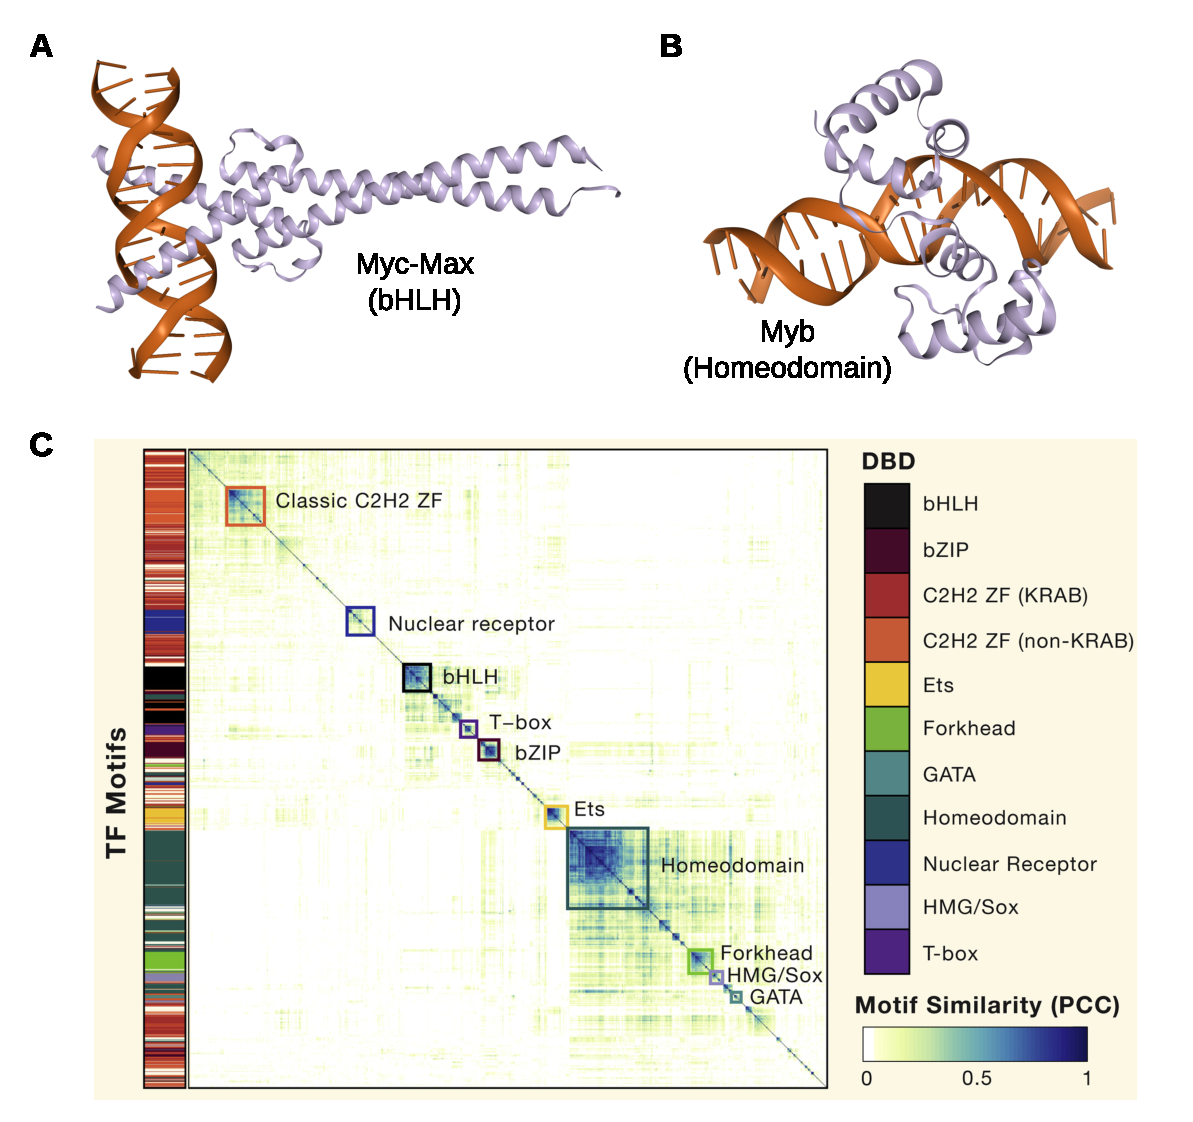
\includegraphics[width=1\textwidth]{figures/dbd_classification/dbd_classification_latest.pdf}
      \caption[TF-DNA binding and TF classification]{\textbf{.} \textbf{A.} . \textbf{B.} Based on their DBD similarity are classified. Often TFs with similar DBDs are binding to highly similar DNA motifs. For example, when performing TF motif pairwise comparison, human TF motifs are grouping according to their DBDs. Adapted from \cite{lambert2018human}.}
      \label{dbd_classification}
    \end{figure}



      \subsubsection{Protein domains}






      \subsubsection{Classification}

        DNA binding domains are highly conserved, thus are used to classify these proteins into families and classes.

        One of the most extensive classification of mammalian transcription factors - TFClass - include superclass, class, family, subfamily and genus \cite{wingender2018tfclass, wingender2013criteria}.





        Many repressor TFs, such as REST, belong to zinc-finger TF family \cite{pang2023identification}.



  \section{Transcription factor binding}


    Transcription factors directly or indirectly bind genomic regions, known as promoters and enhancers. The location where TF resides onto DNA is referred to as a transcription factor binding site (TFBS). A promoter or an enhancer can have multiple TFBSs of the same or different TF. Transcription factors generally have binding preference to a set of DNA sequences - DNA binding motif \cite{boeva2016analysis}.


    
Hopping, scanning, etc from this paper: https://pubmed.ncbi.nlm.nih.gov/25333780/



    \subsection{Transcription factor DNA binding models}

      In order to interpret TF binding to the regulatory regions, we need ways to represent the DNA binding. Currently, DNA binding is represented using various models.


      The most popular and widely used is positional weight matrix (PWM) or position-specific scoring matrix (PSSM). 


      PFM, PWM. Other models to represent binding.





      There are two main strategies applied to analyse genomic sequences from TF binding perspective. One is to find over-represented sequence motifs using existing collections of DNA binding motifs. The second is to discover over-represented motifs \textit{de novo} \cite{boeva2016analysis}. 


      (As a last sentence) There is a common misconception that all TFs are binding DNA very specifically with little variation. In fact, there are different binding mechanisms that TFs can adapt to regulate gene expression in different scenarios.

        \subsubsection{Motif discovery}



        \subsubsection{Use of TF-DNA binding models}

        There are several resources that store simple TF-DNA binding models in a for of PFMs and PWMs. The biggest and most popular ones include JASPAR, CIS-BP and HOCOMOCO.

        TF-DNA binding models can be used to predict putative TFBSs in the genome, using motif scanning tools, such as PWMScan \cite{weidemuller2021transcription}. However, it is known that genome scanning with a motif of interest results in numerous false positives, known as futility theorem \cite{wasserman2004applied}. Therefore, it can be challenging to identify the functional TF binding sites.

      \subsection{Mechanisms of transcription regulation by TFs}

      Transcription factors can be classified into activators and repressors, but this grouping is questioned as TFs can either activate or repress depending on the sequence context and available co-factors \cite{lambert2018human}.


      Transcription factors can bind DNA in different ways, varying from direct binding to the DNA (most well studied) to indirect and cooperative binding. For example, transcription factor PU.1 can bind to DNA directly and indirectly. Direct binding of PU.1 to the consensus motif AGGAA leads to transcriptional activation, while indirect binding through a partner GATA1 to the GATA motif may lead to transcriptional repression \cite{boeva2016analysis}.
      
      It is important to understand that protein binding to DNA mechanisms vary. This is essential to increase the complexity in gene transcription regulation, which is a key to development of living organisms.
      
      Scientists started to understand the variability of gene expression regulation mechanisms by inventing and applying a series of experimental and computational methods. The most famous examples include chromatin immunoprecipitation followed by sequencing (ChIP-seq) and \textit{de novo} motif discovery in genomic regions, respectively. Thus, it is important to understand the advantages and disadvantages of these methods.  
      
      
      
      In this section I will review these binding mechanisms.


      (Go from the simplest to more complicated....)

        \subsubsection{Direct and indirect TF binding}


ChIP-seq, SELEX methods here. Aim to get the DNA pattern, motif, that is directly bound by the TF. What we get is a bit of another story.


Current experimental techniques aim to identify direct TF binding, but in practice, the data reflect direct and indirect TF binding. Indirect can mean that TFs are binding through other TFs. It is still important information. However, then it is challenging to separate the two signals computationally. One method that was developed to identify TFBSs that are directly bound by the TF of interest is ChIP-eat. The method analyses ChIP-seq peaks. \cite{puig2021unibind,gheorghe2019map}


        \subsubsection{Cooperative transcription factor binding}





        Current models of enhancer activity: enhanceosome, billboard and collective TF binding \cite{spitz2012transcription}.


        When TFs interact or compete with each other binding sites co-localize or overlap \cite{boeva2016analysis}.


        Cooperative binding does not always mean that two TFs will bind the DNA directly, they can be cooperating through protein-protein interactions or binding DNA indirectly \cite{mitsis2020transcription}.






        Notes: talk about mechanisms of binding and methods that investigate these mechanisms can be explained here too.
        So this needs to be quite specific mechanisms and then specifics on the methods as well (experimental and computational methods that is).

      \subsection{Impact of methylation to the DNA binding}

% This paper and also to make figure:

%       https://www.science.org/doi/10.1126/science.aaj2239


        \subsubsection{Pioneering}

      TFs are capable of binding heterochramatin through recruitment of histone acetyltransferases \cite{boeva2016analysis}.

